%%%%%%%%%%%%%%%%%%%%%%%%%%%%%%%%%%%%%%%%%
% University/School Laboratory Report
% LaTeX Template
% Version 3.1 (25/3/14)
%
% This template has been downloaded from:
% http://www.LaTeXTemplates.com
%
% Original author:
% Linux and Unix Users Group at Virginia Tech Wiki 
% (https://vtluug.org/wiki/Example_LaTeX_chem_lab_report)
%
% License:
% CC BY-NC-SA 3.0 (http://creativecommons.org/licenses/by-nc-sa/3.0/)
%
%%%%%%%%%%%%%%%%%%%%%%%%%%%%%%%%%%%%%%%%%

%----------------------------------------------------------------------------------------
%	PACKAGES AND DOCUMENT CONFIGURATIONS
%----------------------------------------------------------------------------------------

\documentclass{article}

\usepackage[version=3]{mhchem} % Package for chemical equation typesetting
\usepackage{siunitx} % Provides the \SI{}{} and \si{} command for typesetting SI units
\usepackage{graphicx} % Required for the inclusion of images
\usepackage{natbib} % Required to change bibliography style to APA
\usepackage{amsmath} % Required for some math elements
\usepackage{mathrsfs} 
\usepackage{enumerate} % Required for the enumerate function
\usepackage[siunitx]{circuitikz} % Required for the drawing of circuit diagrams
\usepackage{caption}
\usepackage{graphicx}
\usepackage{subcaption}
\usepackage{xfrac}
\usepackage{float}
\usepackage{enumitem}
\usepackage{chemgreek}
\usepackage{pgfplots}
\usepackage[margin=0.75in]{geometry}
\usepackage{epstopdf}

\setlength\parindent{0pt} % Removes all indentation from paragraphs

\renewcommand{\labelenumi}{\alph{enumi}.} % Make numbering in the enumerate environment by letter rather than number (e.g. section 6)

%\usepackage{times} % Uncomment to use the Times New Roman font

%----------------------------------------------------------------------------------------
%	DOCUMENT INFORMATION
%----------------------------------------------------------------------------------------

\title{Instrumentation \\ Computer Simulation Assignment \\ ENG342} % Title

\author{Shane \textsc{Reynolds}} % Author name

\date{\today} % Date for the report

\begin{document}

\maketitle % Insert the title, author and date

\begin{center}
\begin{tabular}{l r}
Professor: & Dr Suresh Thennadil % Instructor/supervisor
\end{tabular}
\end{center}

% If you wish to include an abstract, uncomment the lines below
% \begin{abstract}
% Abstract text
% \end{abstract}

\tableofcontents
\newpage

%----------------------------------------------------------------------------------------
%	SECTION 1
%----------------------------------------------------------------------------------------

\section{Objective}

An ideal tank heating process scenario will be mathematically modelled. Comparison the model will compared to simulated results, and discussed.

%----------------------------------------------------------------------------------------
%	SECTION 2
%----------------------------------------------------------------------------------------

\section{Background \& Model Derivation}
Consider a tank with a capacity of 1000$\si{\liter}$, which has some feed with a volumetric flow rate for the feed of 200$\si{\litre\per\minute}$, both in and out of the tank. Further, to this the tank is heated with an electric heater. Assuming that there is no heat transfer through the tank walls, the law of conservation of energy suggests that:
\begin{align}
\Bigg[\parbox{3cm}{Rate of heat from incoming liquid}\Bigg] - \Bigg[\parbox{3cm}{Rate of heat form outgoing liquid}\Bigg] + \Bigg[\parbox{3cm}{Rate of heat into tank from heater}\Bigg] = \Bigg[\parbox{3cm}{Rate of heat accumulation in tank}\Bigg]
\end{align}

Heat energy, $Q$, for a liquid is given by the expression:
\begin{align}
Q = m \cdot C_p \cdot (T - T_{ref}),
\end{align}
where is heat energy, $m$ is mass, $C_p$ is specific heat capacity, $T$ is temperature, and $T_{ref}$ is a reference temperature. Rates of heat into the tank due the feed can be found from derivative of (2) with respect to time.
\begin{align}
q_{in} = \frac{dm_{in}}{dt} \cdot C_p \cdot (T_i - T_{ref}),
\end{align}
where $T_i$ is the input temperature from the feed. Similarly, we find the rate of heat out of the tank from the output as:
\begin{align}
q_{out} = \frac{dm_{out}}{dt} \cdot C_p \cdot (T - T_{ref})
\end{align}

The accumulation of heat in the tank, $Q_T$, for a fixed mass, $M$, is given by the following relationship:
\begin{align*}
Q_{T} = M \cdot C_P \cdot (T - T_{ref})
\end{align*}

Differentiating this expression, we get the rate of heat change in the tank accumulation is given by:
\begin{align}
q_{T} = M \cdot C_P \cdot \frac{dT}{dt} = \rho \cdot V \cdot C_P \cdot \frac{dT}{dt}
\end{align}

Substituting equations (3), (4), and (5) into equation (1), we get the following expression:
\begin{align*}
\frac{dm_{in}}{dt} \cdot C_p \cdot (T_i - T_{ref}) - \frac{dm_{out}}{dt} \cdot C_p \cdot (T - T_{ref}) + q_h = \rho \cdot V \cdot C_P \cdot \frac{dT}{dt}
\end{align*}

Noting that $\omega = \frac{dm_{in}}{dt} = \frac{dm_{out}}{dt}$, we can write:
\begin{align}
\omega \cdot C_p \cdot (T_i - T_{ref}) - \omega \cdot C_p \cdot (T - T_{ref}) + q_h = \rho \cdot V \cdot C_P \cdot \frac{dT}{dt}
\end{align}

Considering, this equation in the steady state, yields:
\begin{align}
\omega \cdot C_p \cdot (T_{is} - T_{ref}) - \omega \cdot C_p \cdot (T_s - T_{ref}) + q_h = 0
\end{align}

Subtracting equation (7) from equation (6) yields a first order differential equation in terms of deviation temperature, $T'(t)$:
\begin{align*}
\omega \cdot C_p \cdot T_i'(t) - \omega \cdot C_p \cdot T'(t) + q_h'(t) = \rho \cdot V \cdot C_P \cdot s \cdot T'(t)
\end{align*}

Rearranging, and taking the Laplace transform yields the following equation which describes the behaviour of the plant:
\begin{align}
T'(s) = \bigg(\frac{1}{\tau s + 1}\bigg) \cdot T'_i(s) + \bigg(\frac{R}{\tau s + 1}\bigg) \cdot q'_h(s),
\end{align}

where the time constant and resistance are defined as follows:
\begin{align*}
\tau = \frac{\rho \cdot V}{\omega} \quad \quad R = \frac{1}{\omega \cdot C_P}
\end{align*}
%----------------------------------------------------------------------------------------
%	SECTION 3
%----------------------------------------------------------------------------------------

\section{Time Response of Open Loop System}
Equation (8) defined the theoretical model of the system as:
\begin{align*}
T'(s) = \bigg(\frac{1}{\tau s + 1}\bigg) \cdot T'_i(s) + \bigg(\frac{R}{\tau s + 1}\bigg) \cdot q_h(s)
\end{align*}

In order to specify the model fully, the time constant, $\tau$, and the resistance, $R$, need to be calculated. If the tank capacity, $V$, is 1000$\si{\liter}$, the fluid density, $\rho$, is 1$\si{\kilogram\per\liter}$, and the volumetric flow rate, $v_f$, is 200$\si{\liter\per\minute}$, then the time constant, $\tau$, is determined as:
\begin{align*}
\tau = \frac{\rho \cdot V}{\omega} = \frac{\rho \cdot V}{\rho \cdot \omega} = \frac{1000}{200} = 5\si{\minute}
\end{align*}

The resistance is determined as:
\begin{align*}
R = \frac{1}{\omega \cdot C_P} = \frac{1}{\rho \cdot v_f \cdot C_P} = \frac{1}{836.8}\si{\minute\degreeCelsius\per\kilo\joule}
\end{align*}

\subsection{Plant Time Response for Step Increase in Feed Temperature, With Heat Input Held Constant}
Holding the heat input to the system constant, a step increase in the feed temperature was input to the system. The mathematical model in the Laplace domain can be seen in equation (9):
\begin{align}
T'(s) = \frac{1}{5 \cdot s + 1} \cdot T'_i(s)
\end{align} 

Given a deviation in the input temperature, $T'_i(t)$ , of 10$\si{\degreeCelsius}$, we note that the Laplace transform is:
\begin{align*}
\mathscr{L}\{T'_i(t)\} &= \mathscr{L}\{10 \cdot u(t)\}\\
T'_i(s) &= \frac{10}{s}
\end{align*}

The mathematical model, in the Laplace domain, becomes:
\begin{align}
T'(s) = \frac{10}{s \cdot (5 \cdot s + 1)}
\end{align}

Solving equation (10) yields the following expression for the temperature deviation in the time domain:
\begin{align}
T'(t) = 10 \cdot (1 - e^{-\sfrac{t}{5}})
\end{align}

The plot of this model can be seen in Figure 2. A simulation of the system was run in Simulink using the block diagram shown in Figure 1. The step input, and simulated system response can be seen in Figure 3. It is noted that the model and simulation shown in Figures 2 and 3 are identical.

\begin{figure}[h]
\centering
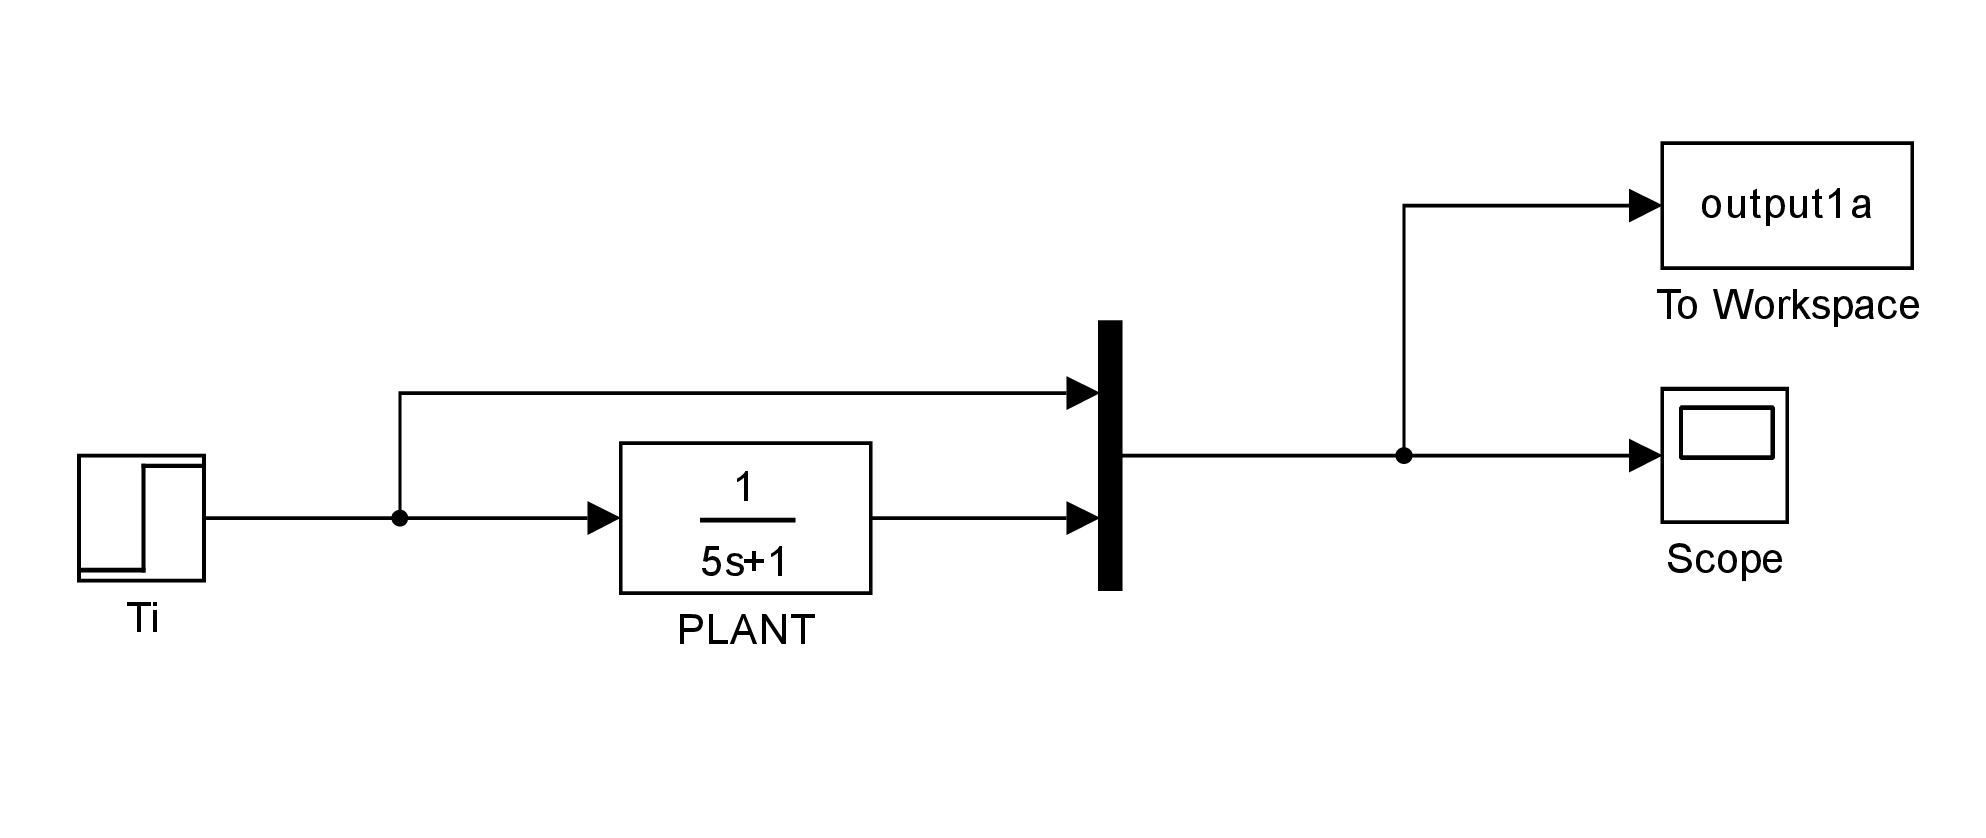
\includegraphics[scale=0.15]{block_1a}
\caption{A block diagram of the plant with a simulated step increase of 10$\si{\degreeCelsius}$ to the feed.}
\end{figure}

\begin{figure}[h]
\begin{minipage}{0.45\textwidth}
\centering
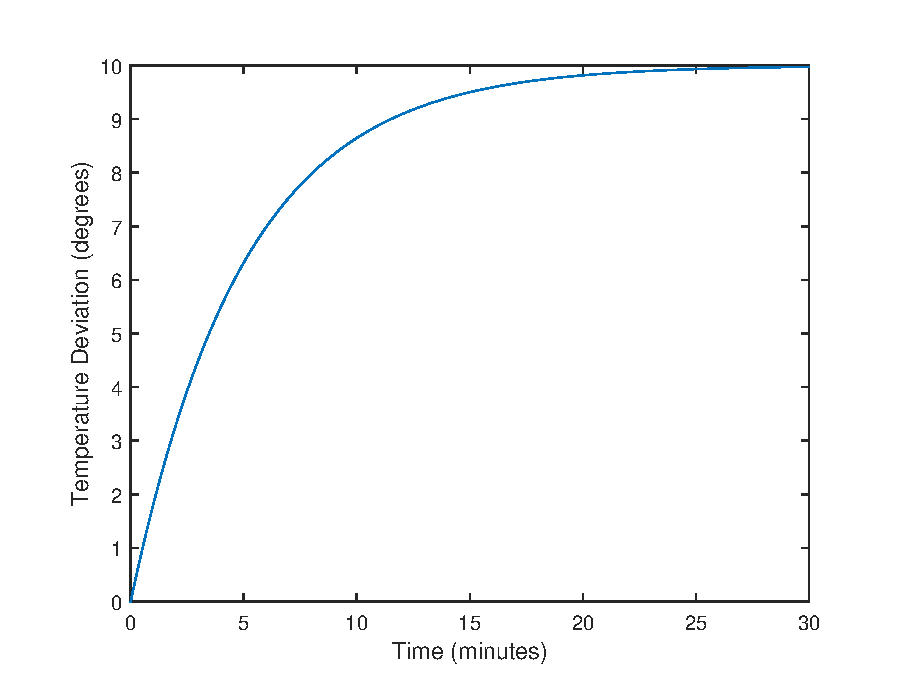
\includegraphics[height=6cm]{1a_mod}
\caption{Temperature deviation model, shown in equation (11), for a step change in the feed temperature of 10$\si{\degreeCelsius}$, holding the heat input constant}
\end{minipage}
\hspace{1cm}
\begin{minipage}{0.45\textwidth}
\centering
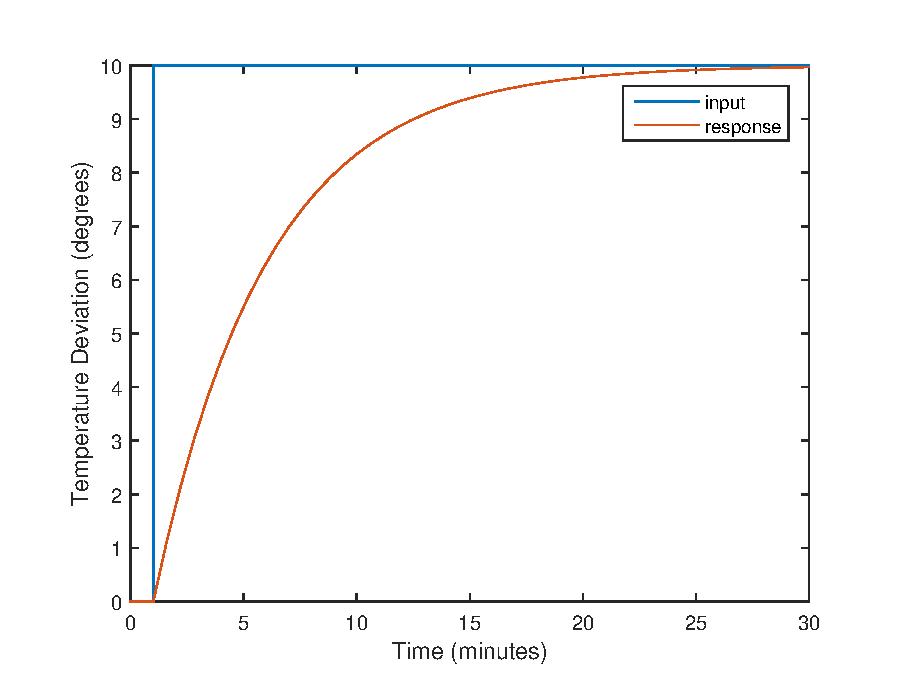
\includegraphics[height=6cm]{1a_sim}
\caption{Temperature deviation simulation for a step change in the feed temperature of 10$\si{\degreeCelsius}$, holding the heat input constant}
\end{minipage}
\end{figure}

\subsection{Plant Time Response for Step Increase in Heat Input, With Feed Temperature Held Constant}
Holding the feed temperature to the system constant, a step increase in the heat input introduced to the system. The mathematical model in the Laplace domain can be seen in equation (12):
\begin{align}
T'(s) = \frac{\sfrac{1}{836.8}}{5 \cdot s + 1} \cdot q'_h(s)
\end{align} 

Given a deviation in the heat input, $q'_h(t)$ , of 42$\si{\kilo\watt} = 2520\si{\kilo\joule\per\minute}$ we note that model shown in equation (12) can be re-written as:
\begin{align}
T'(s) = \frac{2520}{s \cdot (5 \cdot s + 1)}
\end{align}

Solving this system yields the following expression for the temperature deviation in the time domain:
\begin{align}
T'(t) = 3 \cdot (1 - e^{-\sfrac{t}{5}})
\end{align}

The plot of this model can be seen in Figure 5. A simulation of the system was run in Simulink using the block diagram shown in Figure 4. The step input, and simulated system response can be seen in Figure 6. It is noted that the model and simulation shown in Figures 5 and 6 are identical.

\begin{figure}[h]
\centering
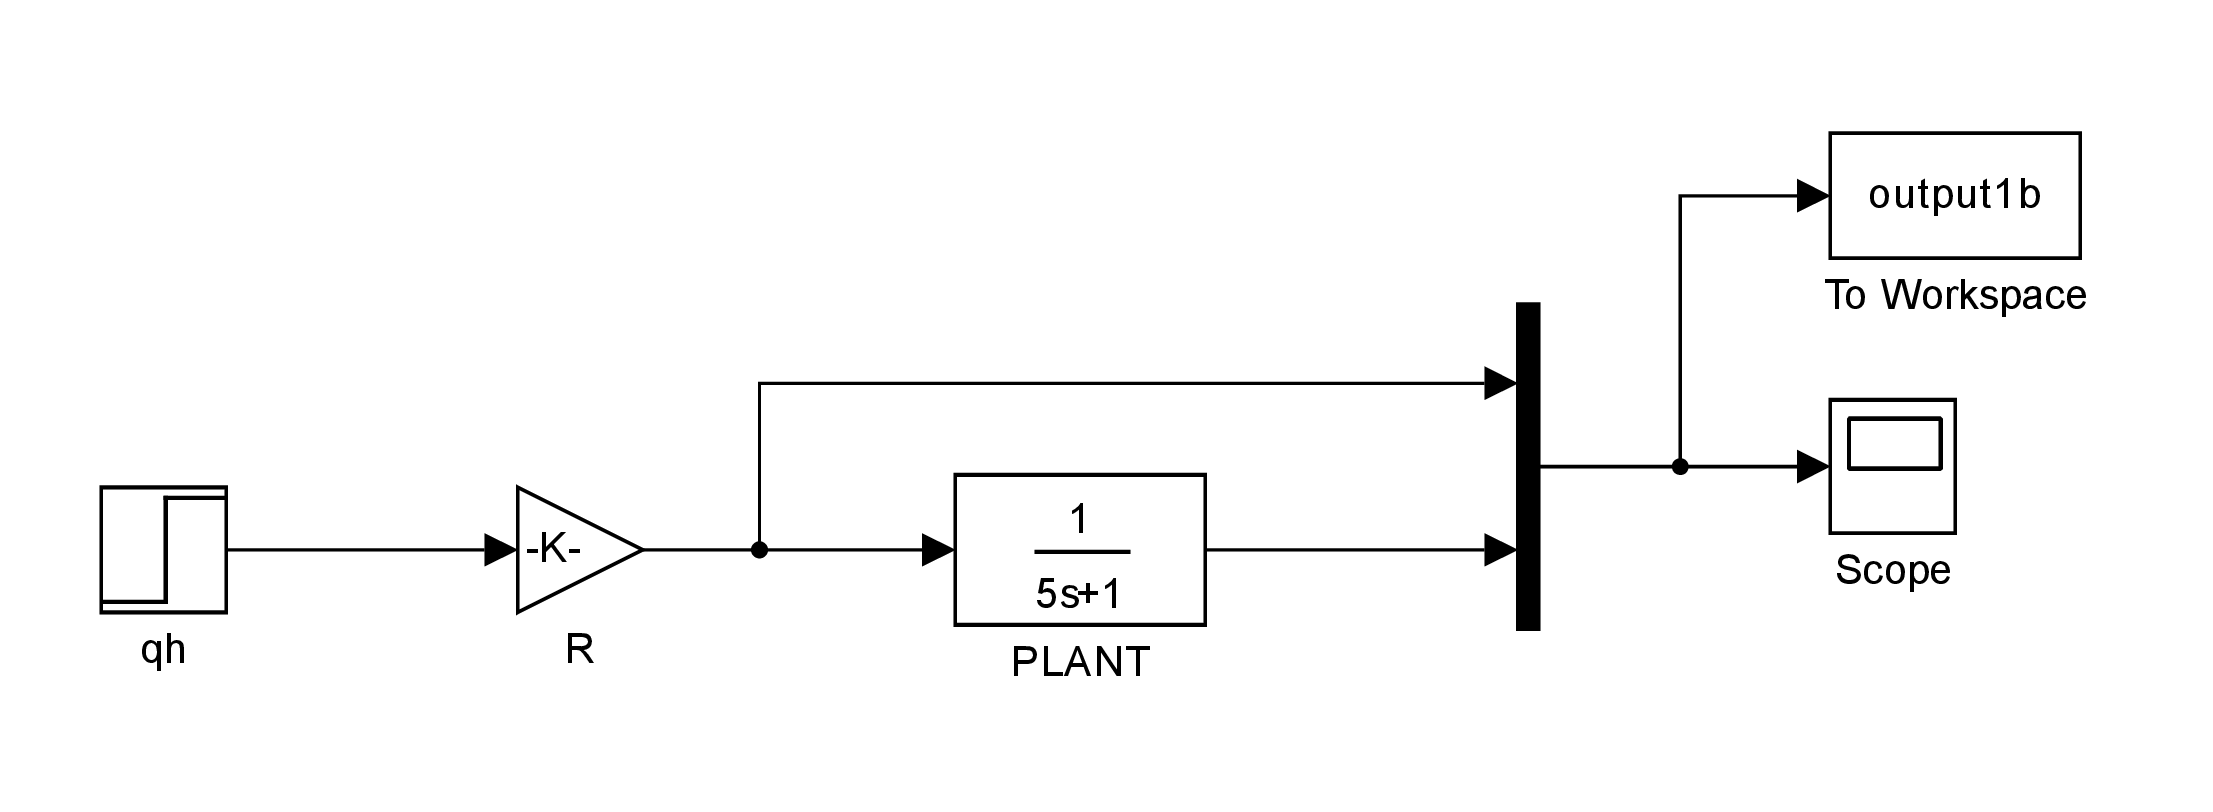
\includegraphics[scale=0.15]{block_1b}
\caption{A block diagram of the plant with a simulated step increase of 42$\si{\kilo\watt}$ to the heat input.}
\end{figure}

\begin{figure}[h]
\begin{minipage}{0.45\textwidth}
\centering
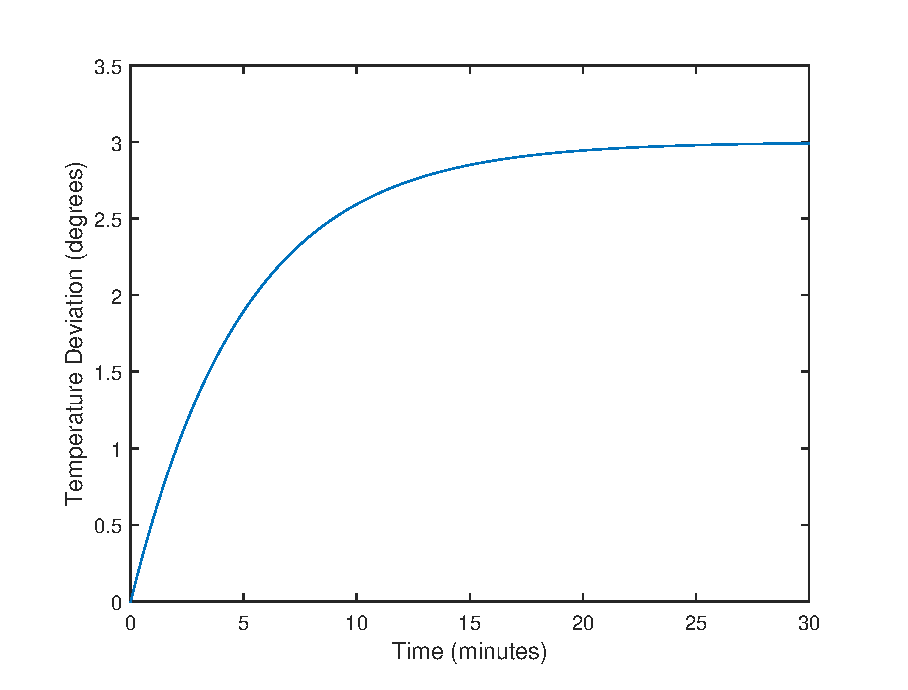
\includegraphics[height=6cm]{1b_mod}
\caption{Temperature deviation model, shown in equation (14), for a step change in the heat input of 42$\si{\kilo\watt}$, holding the feed input temperature constant}
\end{minipage}
\hspace{1cm}
\begin{minipage}{0.45\textwidth}
\centering
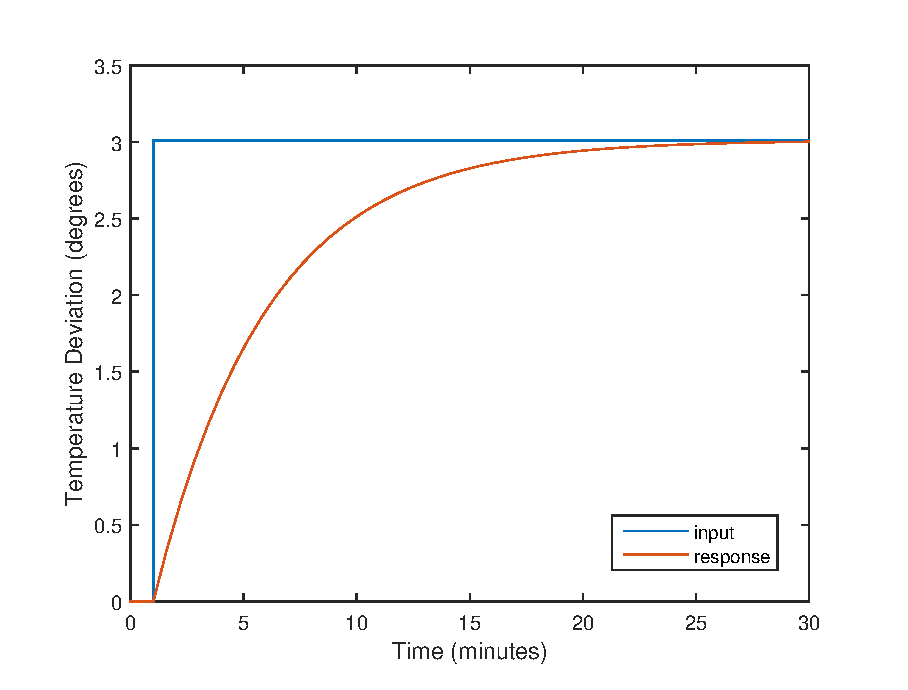
\includegraphics[height=6cm]{1b_sim}
\caption{Temperature deviation simulation for a step change in the heat input of 42$\si{\kilo\watt}$, holding the feed input temperature constant}
\end{minipage}
\end{figure}

\subsection{Plant Time Response for Step Increase in Feed Temperature and Input Heat}

A step increase in the heat input and the feed temperature has the following mathematical model in the Laplace domain:
\begin{align}
T'(s) = \frac{1}{5 \cdot s + 1} \cdot T'_i(s) + \frac{\sfrac{1}{836.8}}{5 \cdot s + 1} \cdot q'_h(s)
\end{align} 

The step increase in the heat from the the feed is 10$\si{\degreeCelsius}$, and the step increase for the heat input is 42$\si{\kilo\watt}$ as seen in the previous two subsections. This yields the following mathematical model in the Laplace domain:
\begin{align}
T'(s) = \frac{10}{s \cdot (5 \cdot s + 1)} + \frac{2520}{s \cdot (5 \cdot s + 1)}
\end{align}

Solving this system yields the following expression for the temperature deviation in the time domain:
\begin{align}
T'(t) = 13 \cdot (1 - e^{-\sfrac{t}{5}})
\end{align}

The plot of this model can be seen in Figure 8. A simulation of the system was run in Simulink using the block diagram shown in Figure 7. The step input, and simulated system response can be seen in Figure 9. It is noted that the model and simulation shown in Figures 8 and 9 are identical.

\begin{figure}[h]
\centering
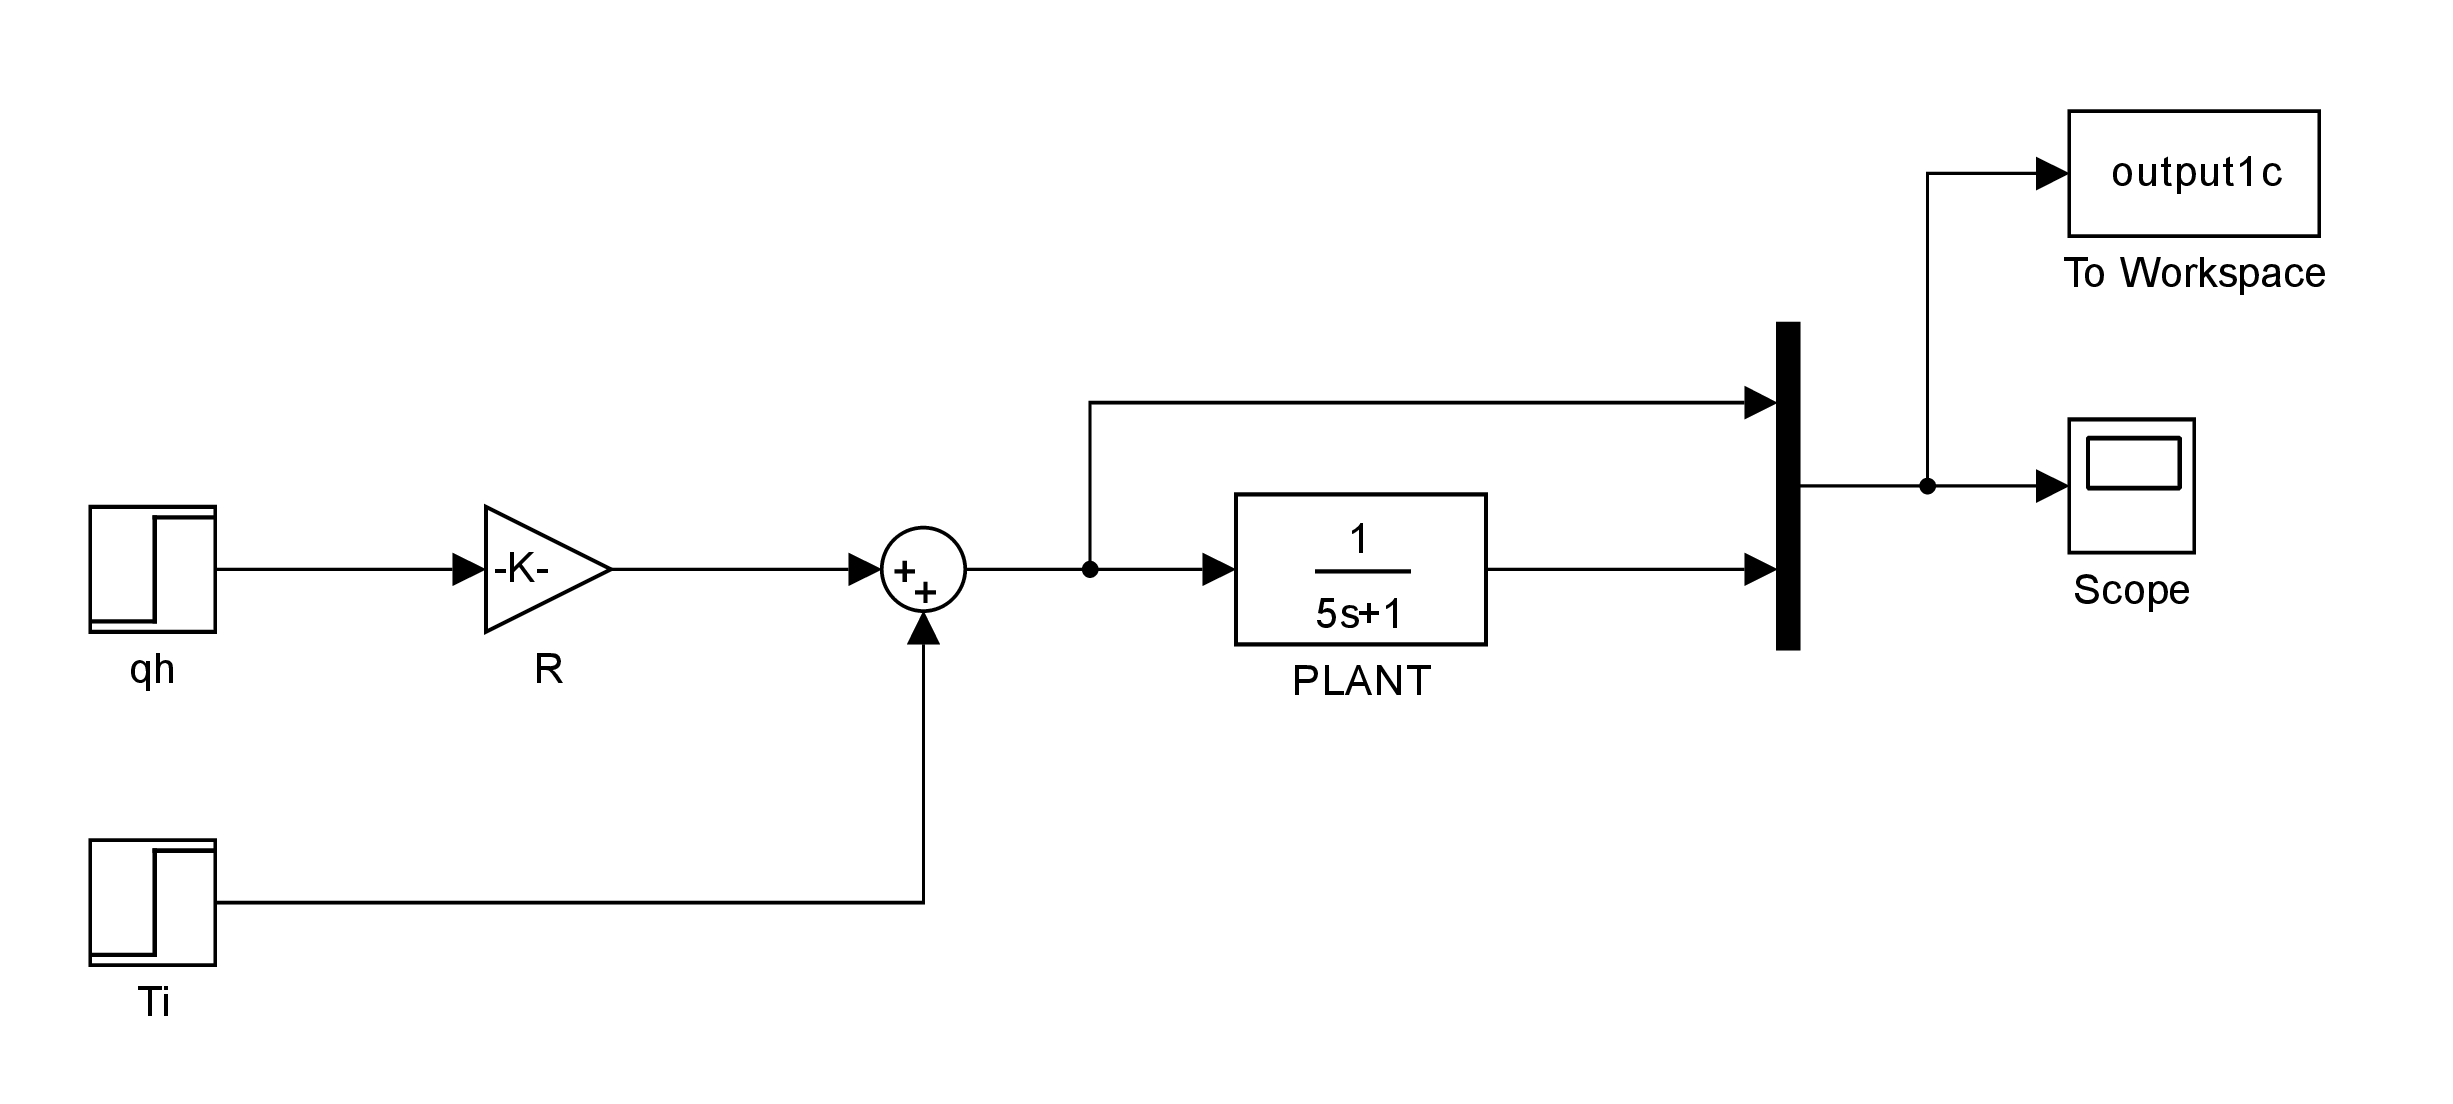
\includegraphics[scale=0.15]{block_1c}
\caption{A block diagram of the plant with a simulated step increase of 10$\si{\degreeCelsius}$ in the feed temperature, and 42$\si{\kilo\watt}$ to the heat input.}
\end{figure}

\begin{figure}[h]
\begin{minipage}{0.45\textwidth}
\centering
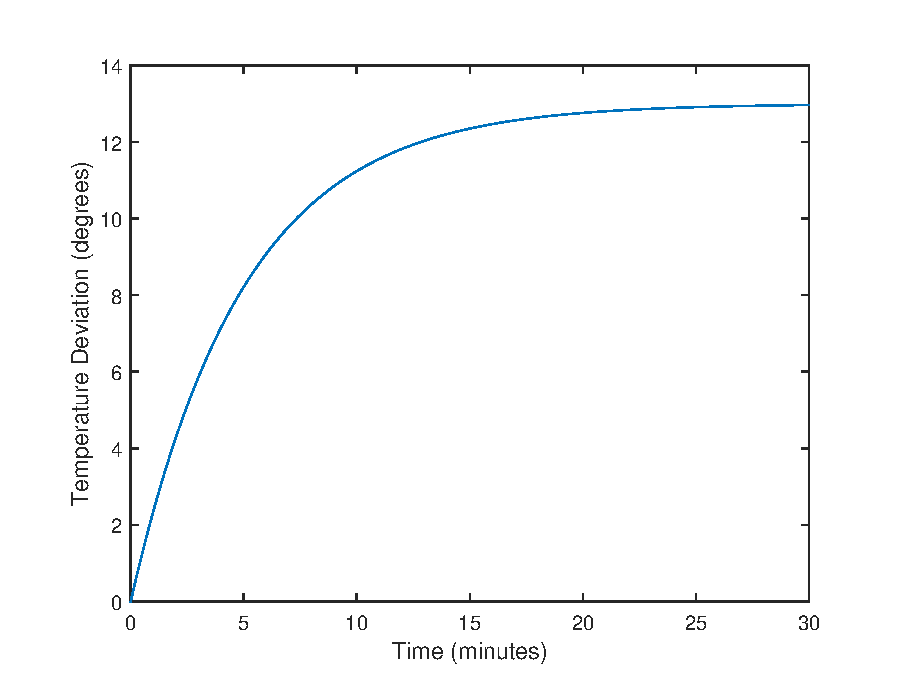
\includegraphics[height=6cm]{1c_mod}
\caption{Temperature deviation model, shown in equation (17), for a step change in the feed temperature of 10$\si{\degreeCelsius}$, and 42$\si{\kilo\watt}$ to the heat input.}
\end{minipage}
\hspace{1cm}
\begin{minipage}{0.45\textwidth}
\centering
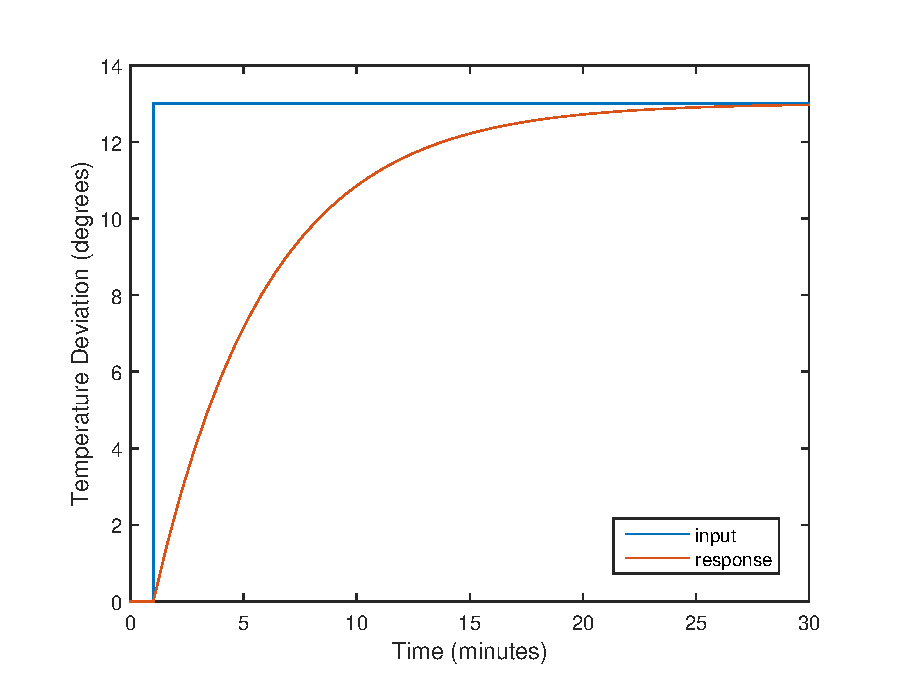
\includegraphics[height=6cm]{1c_sim}
\caption{Temperature deviation simulation for a step change in the feed temperature of 10$\si{\degreeCelsius}$, and 42$\si{\kilo\watt}$ to the heat input.}
\end{minipage}
\end{figure}

The main point of interest is that the step response from a change in feed temp and the step response from a change in heat input are combined to provide the step response for a simultaneous change in both. 

%----------------------------------------------------------------------------------------
%	SECTION 3
%----------------------------------------------------------------------------------------

\section{Instrument Time Response for the Step Increase in Feed Temperature}

The temperature deviation, $T'(t)$, is measured by an instrument which is modelled by a first order system with a time constant of 0.5$\si{\minute}$. The mathematical model, in the Laplace domain, of the temperature deviation measured by the instrument, $T'_m(t)$, is as follows: 
\begin{align*}
T'_m(s) = \bigg(\frac{1}{0.5 s + 1}\bigg) \cdot T'(s) = \bigg(\frac{1}{0.5s + 1}\bigg) \cdot \bigg(\frac{1}{5s + 1}\bigg) \cdot T'_i(s)
\end{align*}

A step increase in the temperature from the the feed of 10$\si{\degreeCelsius}$, yields the following mathematical model in the Laplace domain:
\begin{align*}
T'_m(s) = \frac{10}{s \cdot (0.5s + 1) \cdot (5s + 1)}
\end{align*}

Solving this system yields the following expression for the temperature deviation, as measured by the instrument, in the time domain:
\begin{align}
T'_m(t) = 10 \cdot (1 + 0.11 \cdot e^{-2t} - 1.11 \cdot e^{-0.2t})
\end{align} 

The plot of this model can be seen in Figure 11. A simulation of the system was run in Simulink using the block diagram shown in Figure 10. The step input, and simulated system response can be seen in Figure 12. It is noted that the model and simulation shown in Figures 8 and 9 are identical.\\

\begin{figure}[h]
\centering
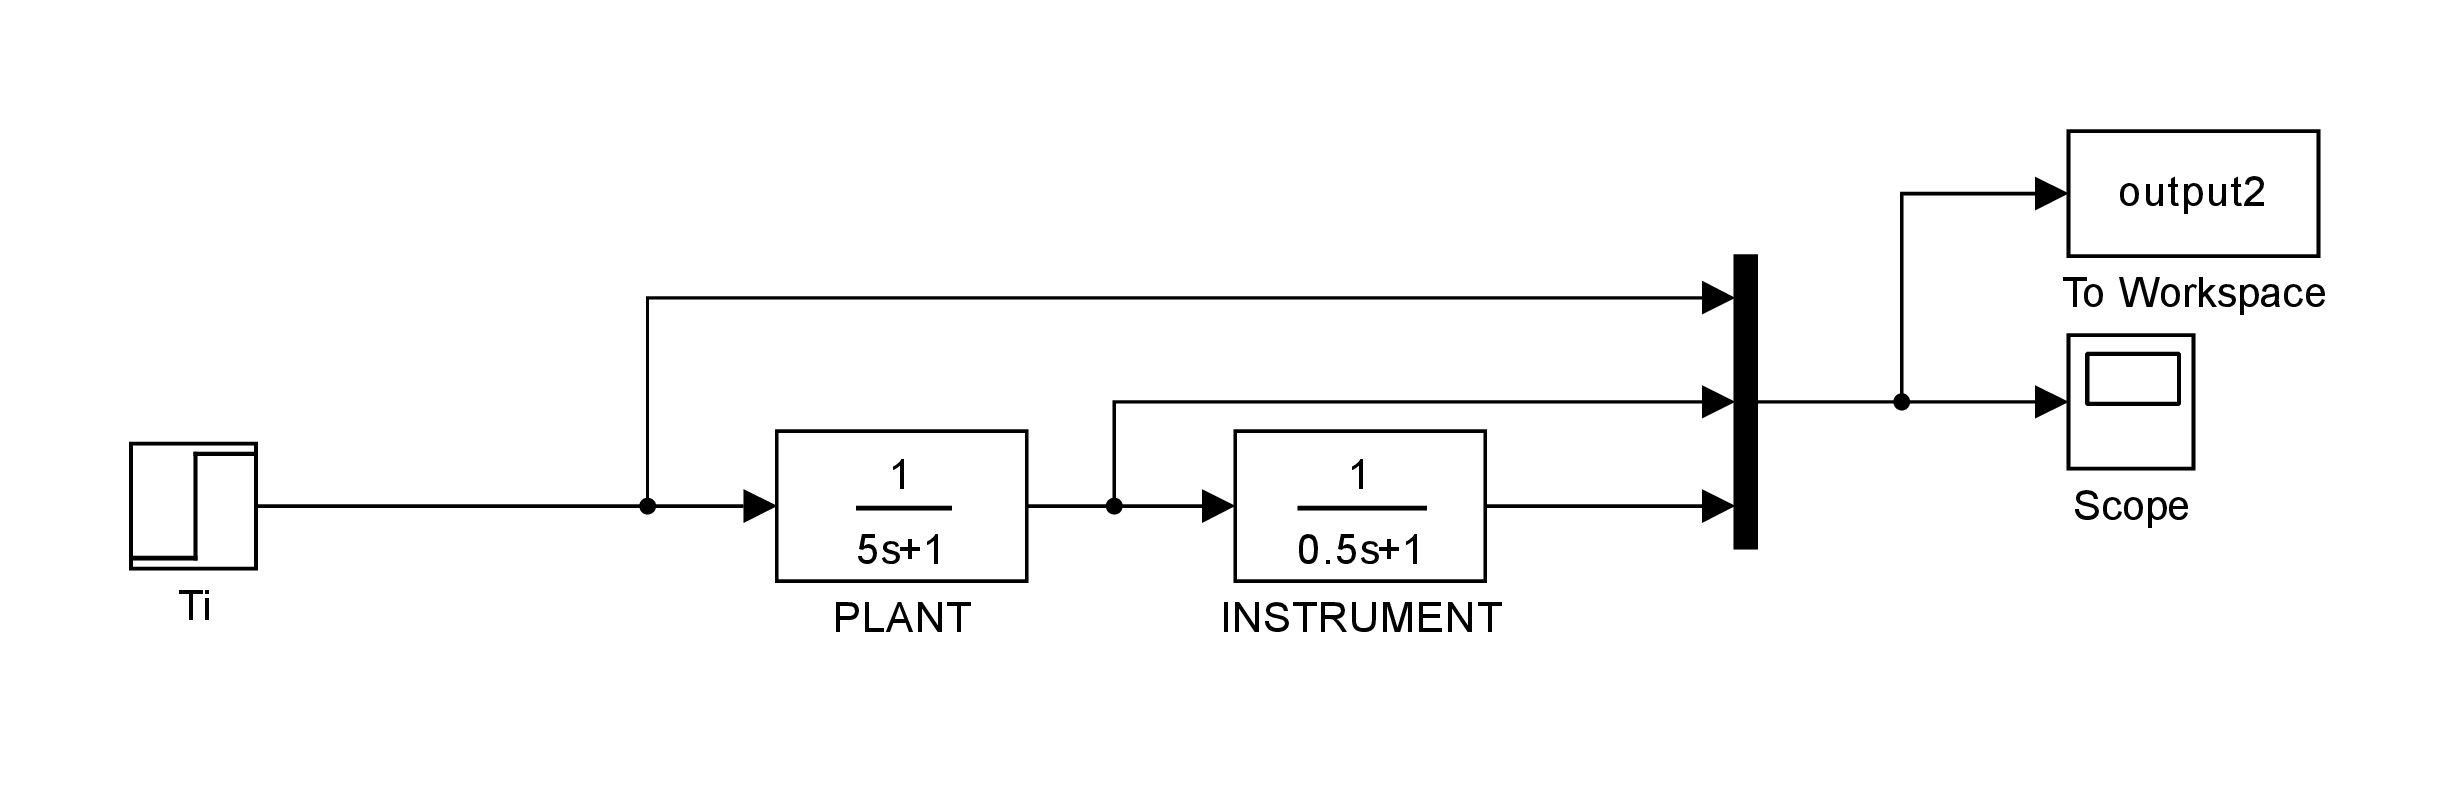
\includegraphics[scale=0.15]{block_2}
\caption{A block diagram of the plant and outlet temperature measurement instrument with a simulated step increase of 10$\si{\degreeCelsius}$ in the feed temperature.}
\end{figure}

\begin{figure}[h]
\begin{minipage}{0.45\textwidth}
\centering
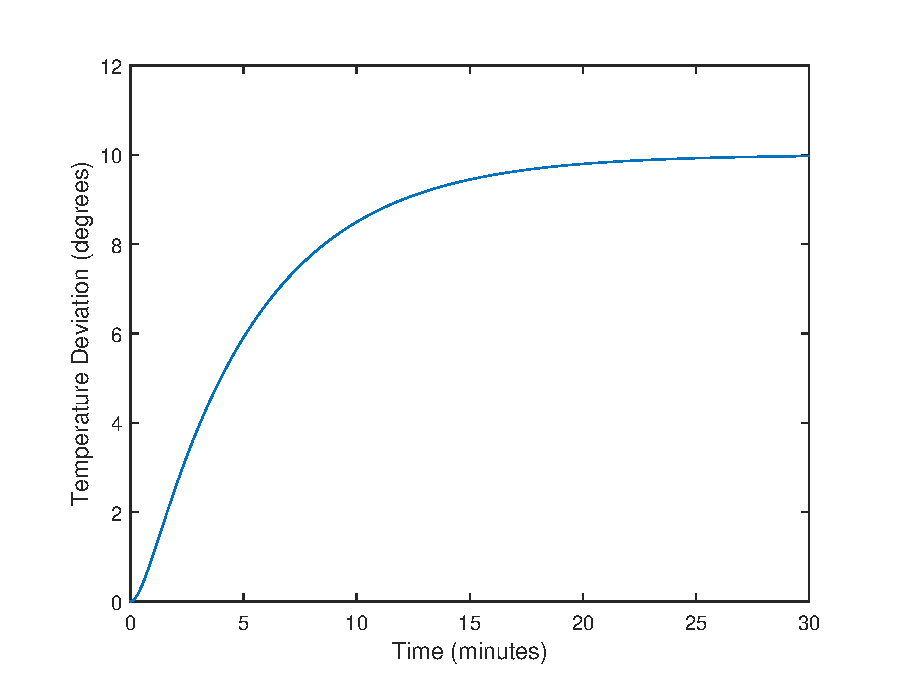
\includegraphics[height=6cm]{2_mod}
\caption{Measured temperature deviation model, shown in equation (18), for a step change in the feed temperature of 10$\si{\degreeCelsius}$, holding the heat input constant}
\end{minipage}
\hspace{1cm}
\begin{minipage}{0.45\textwidth}
\centering
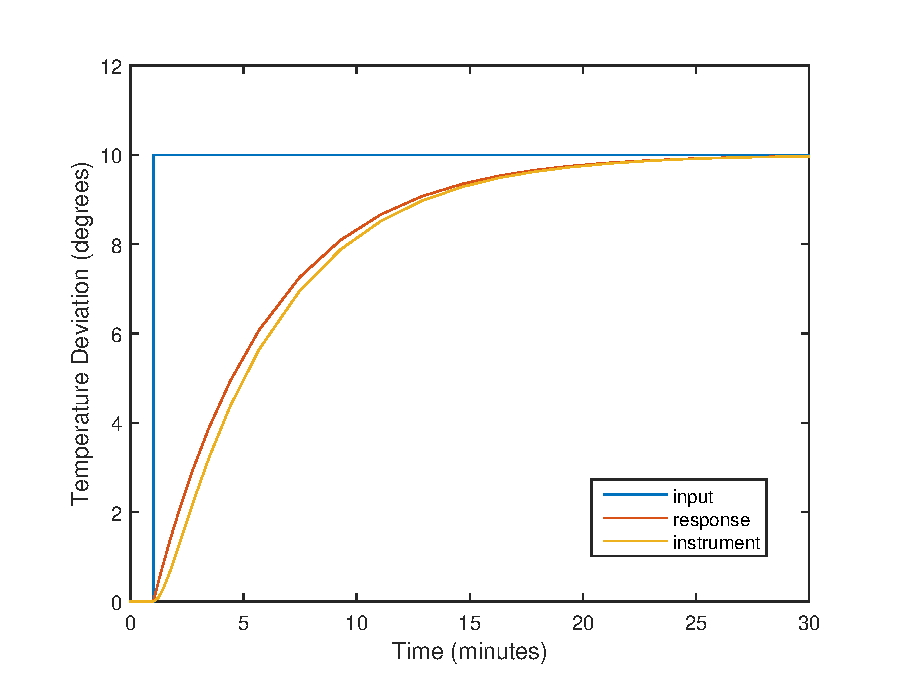
\includegraphics[height=6cm]{2_sim}
\caption{Temperatue deviation and measured temperature deviation simulation for a step change in the feed temperature of 10$\si{\degreeCelsius}$, holding the heat input constant}
\end{minipage}
\end{figure}

Figure 12 shows that there is some measurement error in the initial response to a step change in the feed temperature. This can be seen from the lag in instrument response when compared to the actual outlet temperature. This is in line with expectations as the measurement instrument output goes through two first order systems, as opposed to the actual signal which simply travels through a single first order system. 

%----------------------------------------------------------------------------------------
%	SECTION 4
%----------------------------------------------------------------------------------------

\section{Piping \& Instrumentation Diagram of Tank Heating System}

A piping and instrumentation diagram (P\&ID) describes the process, and how the instrumentation is interconnected. The P\&ID for the tank heating problem can be seen in Figure 13. Notably, there are three instruments in use:
\begin{enumerate}
	\item \textbf{Temperature transmitter}: measures and transmits the temperature electronically to the control room. This instrument is denoted with the symbol TT.
	\item \textbf{Temperature Indicator \& Control}: displays the current tank temperature and sends a control signal to the mechanism which actuates the valve control to let more (or less) steam into the heating element, based on the current state of the system. This instrument is denoted with the symbol TIC.
	\item \textbf{Temperature Computer Output}: receives the control signal from the controller and pneumatically actuates the flow valve to let in more (or less) steam, depending on the control signal. This instrument is denoted with the symbol TY.
\end{enumerate}
\begin{figure}[h]
	\centering
	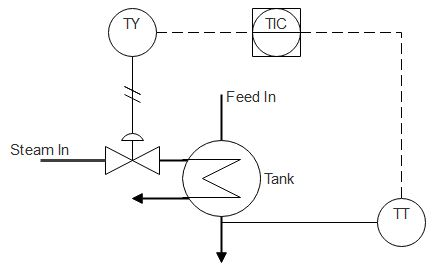
\includegraphics[scale=0.6]{p_id.jpg}
	\caption{Piping and instrumentation diagram for the tank heating system modelled in this report.}
\end{figure}

%----------------------------------------------------------------------------------------
%	SECTION 5
%----------------------------------------------------------------------------------------

\section{PID Controller For Tank Heating System}
A proportional-integral-derivative (PID) controller is fed an error signal $e(t)$. The error signal is defined as the set point minus the process variable. The output of the PID is some signal $u(t)$ which provides input into the system in order to drive the error signal, $e(t)$, towards zero. PID controllers are used in closed loop feedback topologies, as shown in Figure 14.
\begin{figure}[h]
\centering
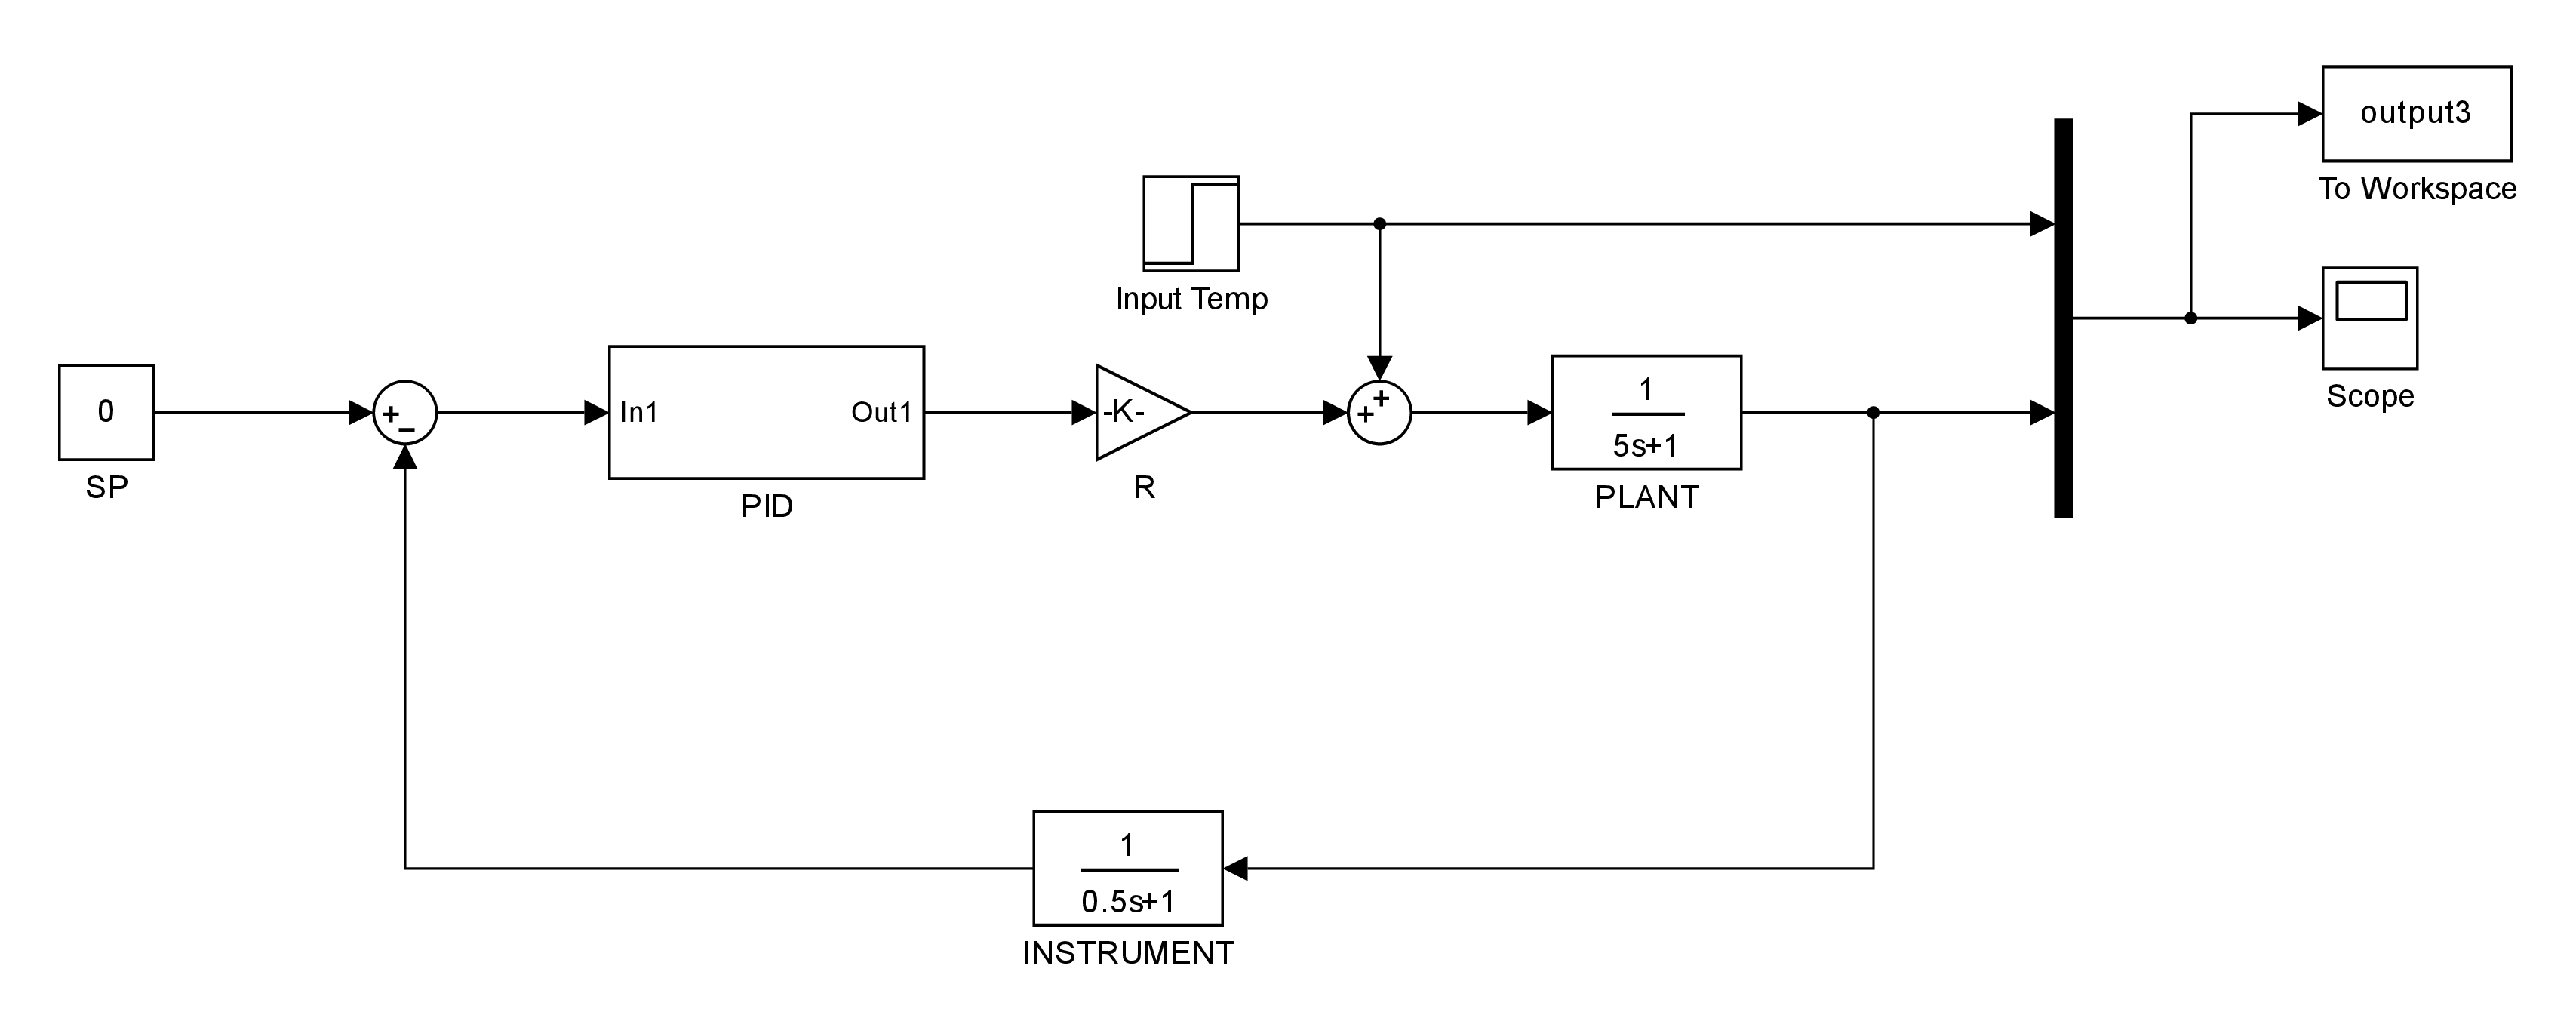
\includegraphics[scale=0.15]{block_45}
\caption{A block diagram of the plant controlled using PID in a feedback topology, with a simulated step increase of 10$\si{\degreeCelsius}$ in the feed temperature.}
\end{figure}

Mathematically, a PID controller is defined as follows:
\begin{align}
u(t) = K_P \cdot e(t) + \frac{K_P}{t_i} \cdot \int_{0}^{t} e(\tau) d\tau + K_P \cdot t_d \cdot \frac{de(t)}{dt}
\end{align}

The parameter $K_P$ is the proportional control parameter. The other two parameters of importance in equation XX are $t_i$, and $t_d$, which are called the integral time and derivative time parameters. Equation XX was implemented in the simulation, as shown in Figure 15.
\begin{figure}[h]
\centering
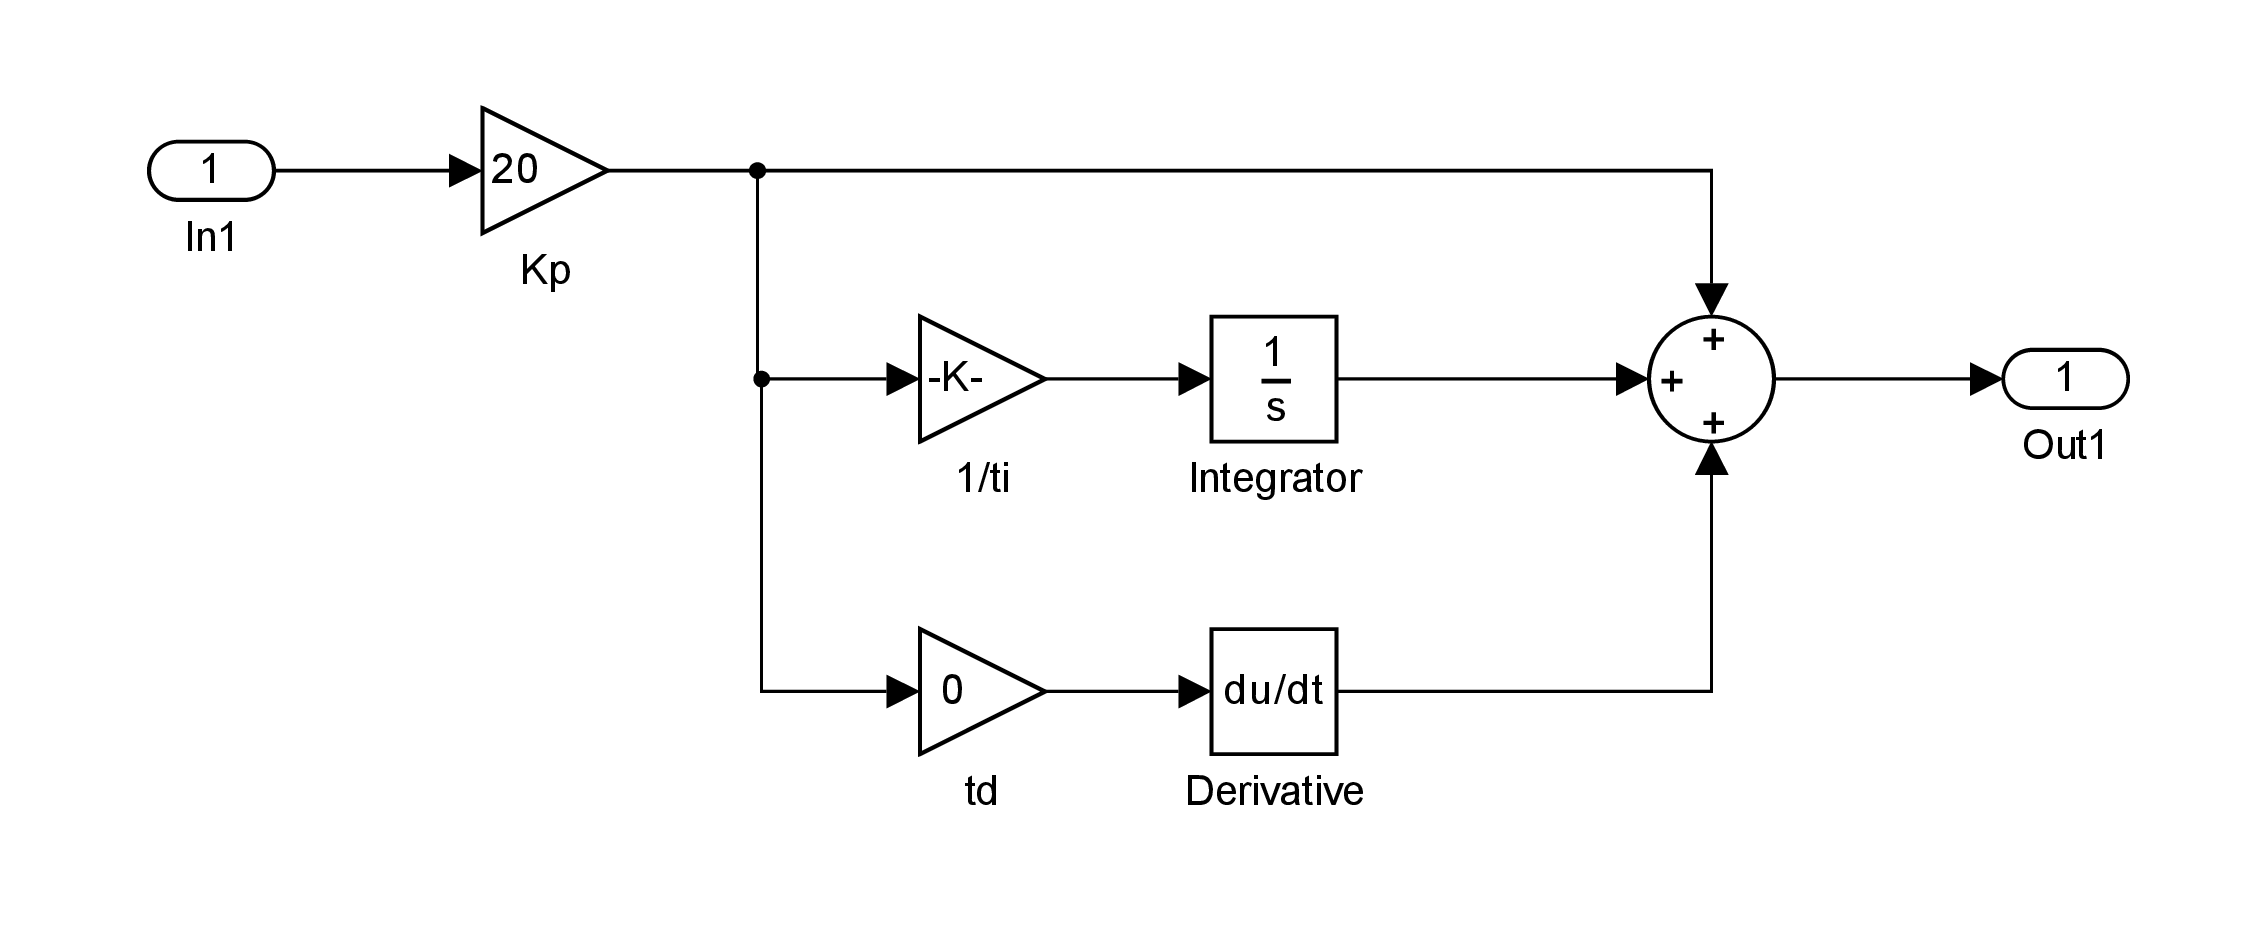
\includegraphics[scale=0.15]{block_3_pid}
\caption{The functional block diagram of the PID implementation.}
\end{figure}
\newpage
%----------------------------------------------------------------------------------------
%	SECTION 5.1
%----------------------------------------------------------------------------------------

\subsection{Proportional (P) Control}
The PID controller, shown implemented in Figure 14, was tuned to provide proportional control only. The proportional gain, $K_P$, was set to 20. Additionally, we let $t_i \rightarrow \infty$, and $t_d = 0$. A step input of 10$\si{\degreeCelsius}$ in the feed of the system was simulated. The results of the simulation can be seen in Figure 16. Figure 17 is a reproduction of Figure 3 for comparison purposes.
\begin{figure}[h]
\begin{minipage}{0.45\textwidth}
\centering
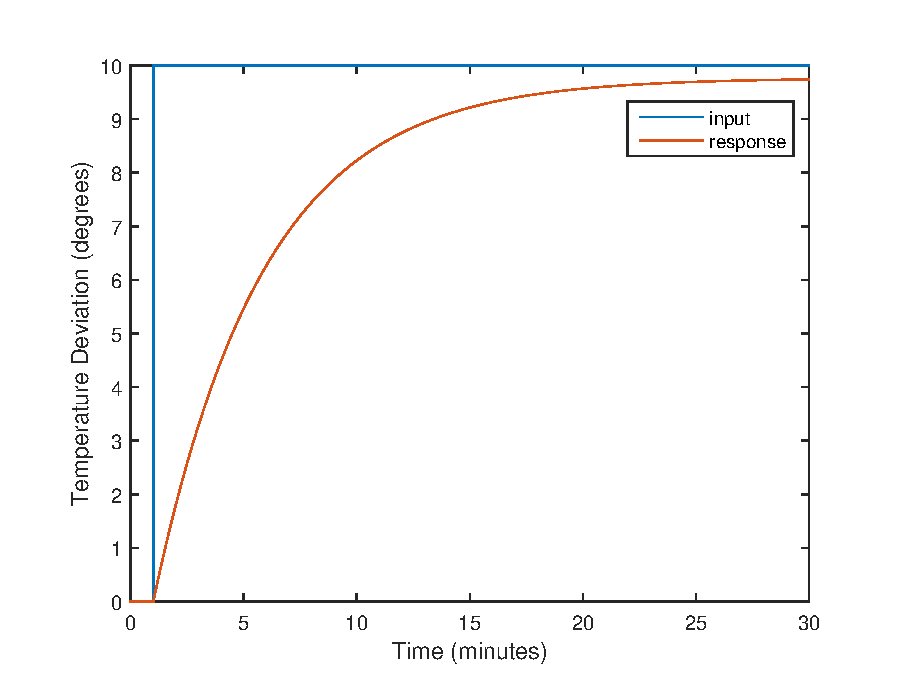
\includegraphics[height=6cm]{3_sim_P}
\caption{Closed loop P feedback control on the tank heating system for a step change in the feed temperature of 10$\si{\degreeCelsius}$}
\end{minipage}
\hspace{1cm}
\begin{minipage}{0.45\textwidth}
\centering
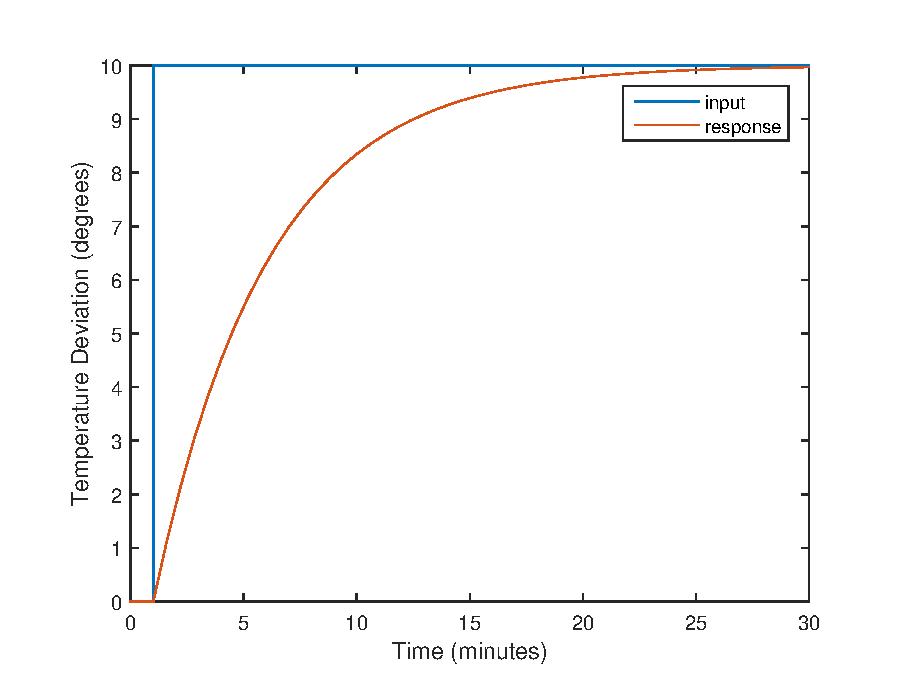
\includegraphics[height=6cm]{1a_sim}
\caption{Open loop temperature deviation simulation for a step change in the feed temperature of 10$\si{\degreeCelsius}$, holding the heat input constant}
\end{minipage}
\end{figure}

Comparison of Figures 16 and 17 show a clear marginal improvement on the response of the system with control implemented. It is the intention of the controller, given some perturbation to the system, to move the system process variable back to the set point. In this instance, perfect control would see the temperature deviation fall down to zero. This has not happened using only proportional control, however, the control measure has slowed the convergence to a deviation temperature to the 10$\si{\degreeCelsius}$ increase. 

%----------------------------------------------------------------------------------------
%	SECTION 5.2
%----------------------------------------------------------------------------------------

\subsection{Proportional Integral (PI) Control}
The proportional gain, $K_P$, was again set to 20. In a series of three simulations $t_i$ was set to equal 0.5$\si{\minute}$, 1$\si{\minute}$, and 1.5$\si{\minute}$. In each of the three simulations, we let $t_d = 0$. A step input of 10$\si{\degreeCelsius}$ in the feed of the system was simulated in each of the three simulations. The simulation results can be seen in Figures 18, 19, and 20, respectively.
\begin{figure}[h]
\begin{minipage}{0.45\textwidth}
\centering
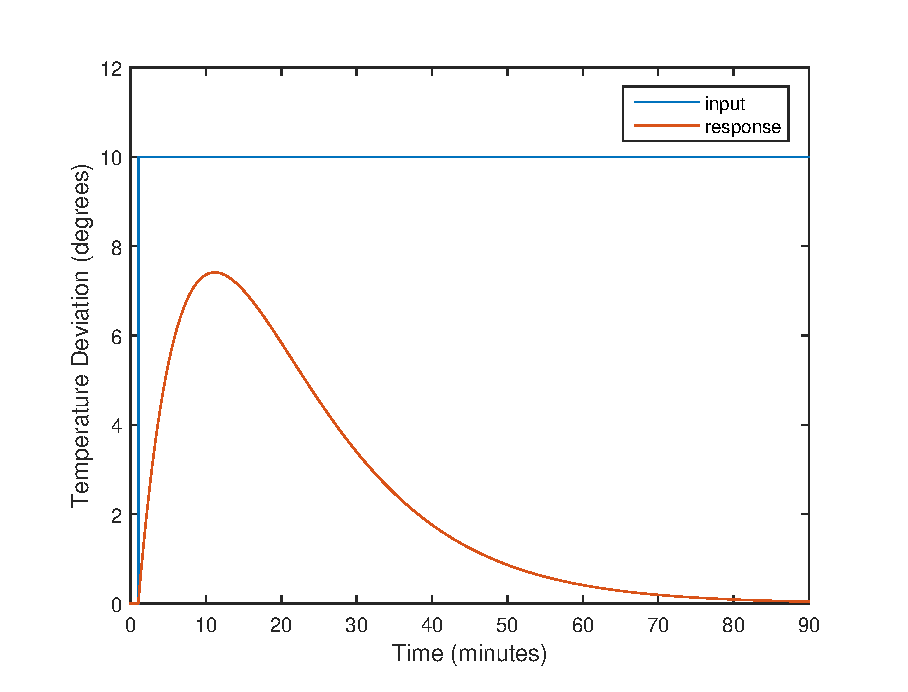
\includegraphics[height=6cm]{3_sim_30}
\caption{Closed loop PI ($t_i=0.5\si{\minute}$) feedback control on the tank heating system for a step change in the feed temperature of 10$\si{\degreeCelsius}$}
\end{minipage}
\hspace{1cm}
\begin{minipage}{0.45\textwidth}
\centering
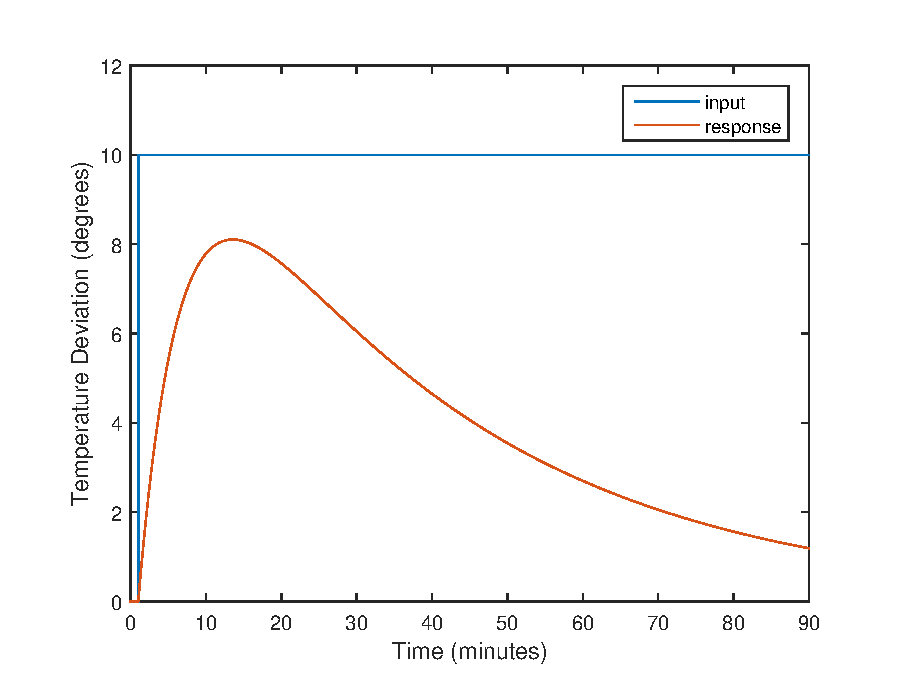
\includegraphics[height=6cm]{3_sim_60}
\caption{Closed loop PI ($t_i=1\si{\minute}$) feedback control on the tank heating system for a step change in the feed temperature of 10$\si{\degreeCelsius}$}
\end{minipage}
\end{figure}
\begin{figure}[h]
\centering
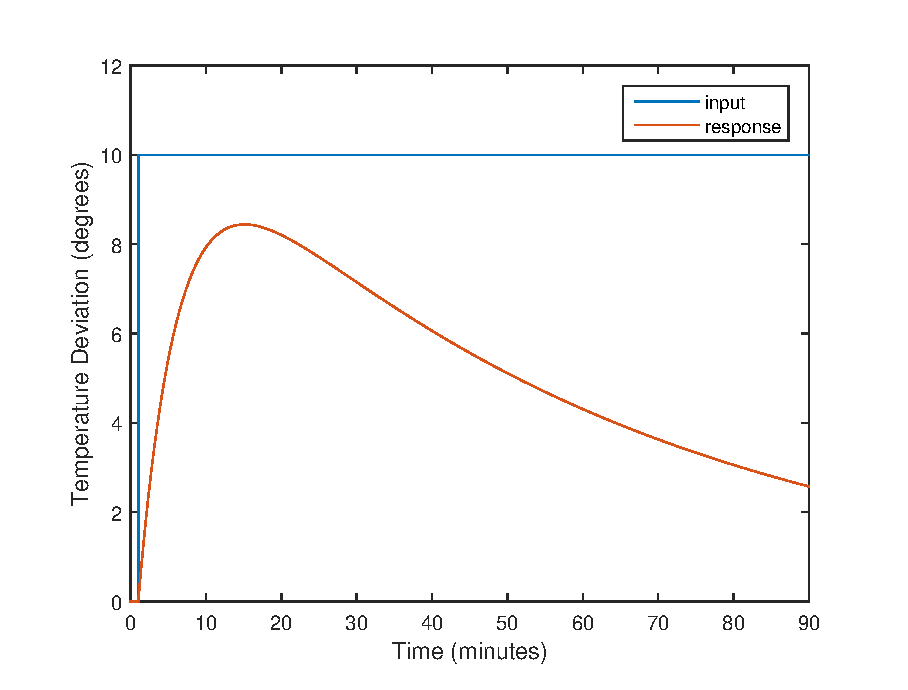
\includegraphics[height=6cm]{3_sim_90}
\caption{Closed loop PI ($t_i=1.5\si{\minute}$) feedback control on the tank heating system for a step change in the feed temperature of 10$\si{\degreeCelsius}$}
\end{figure}

As stated in the previous section, the intention of the controller is to move the controlled process variable to the desired set point. In this case, the process variable is the deviation in the outlet temperature, $T'(s)$. The set point is zero meaning given some perturbation from the feed input, the controller needs to maintain the process at initial conditions. The PI feedback controller show marked improvement over the P feedback controller. This can be seen in Figures 18, 19, and 20. All figures show control towards the desired set point of zero. The best is obviously the controller with $t_i=0.5\si{\minute}$, as this converges the fastest. 
\end{document}